\section{Introduction}
\label{sec:introduction}

An archive can contain several correct descriptions of an attribute from different periods.
A company appoints a new director.
A product changes its supported features.
A policy replaces an earlier threshold.
Retrieval-augmented generation must select the description that applies to the question's date~\citep{lewis2020rag}.
Text similarity identifies the topic, but does not establish that period.

\begin{figure*}[t]
\centering
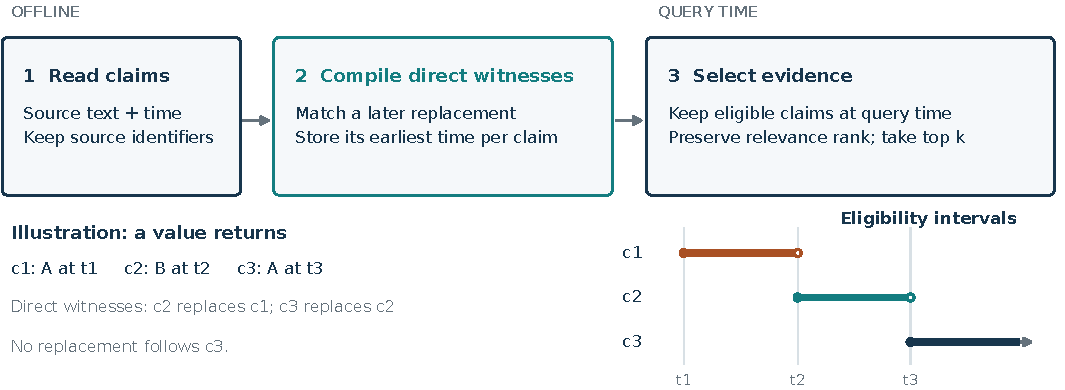
\includegraphics[width=\textwidth]{figures/architecture.pdf}
\caption{Direct certificates connect evidence selection to its replacement sources. The compiler stores the first accepted replacement for each claim. Query-time filtering preserves relevance order before selecting the context. The lower illustration shows a value that returns after replacement. Each occurrence keeps its own interval. Filled endpoints are included; open endpoints are excluded.}
\label{fig:architecture}
\end{figure*}


Consider an illustrative organization, Northstar.
A 2019 record names Mira as its director.
A 2021 record names Leon.
A 2024 record names Sana.
A current question needs Sana's record.
A question about 2022 needs Leon's record.
Both questions search the same archive.
Deleting older records prevents historical answers.
Keeping all relevant records leaves the reader to resolve competing states within a limited context.
The required operation is temporal evidence selection.

One approach groups related claims and orders each group by time.
An earlier statement then expires when another value appears in its group.
This works when every group corresponds to one coherent history.
Text comparisons, however, can connect claims from different subjects or attributes.
If grouping uses connected components, one incorrect connection can merge their histories.
Time ordering can then treat unrelated statements as replacements.
The resulting exclusions can extend beyond the mistaken pair.
They can also change answers about periods before either bridge endpoint existed.

We ask a structural question:
\emph{How can a retrieval memory support historical states while limiting the propagation of comparison errors?}
We study direct supersession certificates.
A certificate connects a claim to its earliest accepted replacement.
Its start and endpoint determine when that claim may enter the reader's context.
Each certificate preserves the source of the replacement decision.
Figure~\ref{fig:architecture} shows the complete selection process.

Direct temporal invalidation already appears in Graphiti~\citep{rasmussen2025zep}.
Our contribution is its formal behavior under arbitrary pairwise decisions.
The matcher can make errors.
Two accepted links need not justify a third link.
We prove that one certificate per claim exactly represents every temporal cutoff.
We also prove that later-dated additions preserve earlier eligibility decisions.
Finally, changing one pair can affect only its older endpoint's interval.
Under fixed relevance scores, the selected set changes by at most one removal and one insertion.
These properties follow from direct dependence on replacement evidence.
They do not require perfect entity resolution.

We implement an exact compiler that scans timestamp batches and retires each claim after finding its first witness.
The compiler receives text, identifiers, and timestamps.
It preserves the supplied matcher while avoiding transitive grouping.
Complete candidate blocking reduces unnecessary comparisons without changing the output.

Our evaluation separates stability from retrieval accuracy.
It tests observed histories, individual pair changes, full-pool evidence selection, and compiler equivalence.
We also inspect the complete answer sets behind TempLAMA~\citep{dhingra2022templama}.
This inspection distinguishes a changed selected answer from an actual removal of the earlier answer.
The resulting protocol evaluates all source-supported answers with unchanged rankings.

The contributions are a formal account of direct invalidation, an exact compiler, and an empirical analysis of temporal error propagation.
The experiments compare direct certificates with component timelines and exact-group date selection under shared extraction and relevance scores.
This design identifies which benefits arise from compilation and which still depend on the matcher.

